\documentclass[a4paper, 12pt]{article}
\usepackage[top=1cm, bottom=1.5cm, left=1cm, right=1cm]{geometry}
\usepackage[utf8]{inputenc}
\usepackage{graphicx, caption}
\usepackage{float}
\usepackage{amsmath, amsfonts, amssymb, esint}
\usepackage{multicol}

\pagenumbering{Roman}

\begin{document}
	\begin{center}
	\begin{large}
		\textbf{Determinação da Viscosidade do Ar}	
	\end{large}
	\end{center}
	
	\begin{center}
		\textit{Iago Mendes, Hugo Alkimim, Gabriel Oliveira Mota, e Marcos Aurélio Duarte Carvalho}
	\end{center}

	\textbf{Resumo}
		\setlength{\parindent}{4ex}
		\par Neste artigo, explora-se um arranjo experimental de um oscilador massa-mola para investigar a oscilação harmônica amortecida. A determinação da amplitude da oscilação como uma função temporal foi determinada precisa e economicamente, utilizando vídeos obtidos por meio de um celular, a ferramenta \textit{Tracker -- Video Analysis and Modeling Tool for Physics Education --} e algoritmos em \textit{MATLAB}. Assim, foi possível determinar o coeficiente de amortecimento, que foi usado para encontrar a viscosidade do ar.
	
	\begin{multicols}{2} \begin{enumerate}
		\item \textbf{Introdução}
			
		\item \textbf{Teoria}
			\setlength{\parindent}{4ex}
			\par Em primeira instância, viscosidade ($\eta$) é a propriedade física que descreve a resistência de um fluido para escoar, que é geralmente expressa usando a Lei de Newton da Viscosidade:
				\begin{figure}[H]
					\centering
					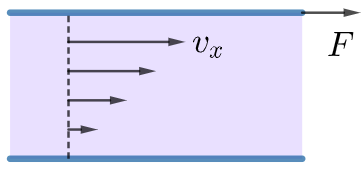
\includegraphics[scale=0.6]{./img/viscosidade.png}
				\end{figure}
				$$\frac{F}{A} = \eta \dfrac{dv_x}{dy}$$
				em que $F$ é a força aplicada, $A$ é a área em $y$ e $z$, e $\dfrac{dv_x}{dy}$ é a derivada espacial da velocidade. No Sistema Internacional, a viscosidade possui \textit{pascal-segundo} [$Pa \cdot s$] como unidade de medida.
				\par Além disso, quando estudamos a mecânica de fluidos, devemos sempre considerar o número de Reynolds, um coeficiente adimensional utilizado para o cálculo do regime de escoamento de um fluido sobre uma superfície. Esse coeficiente é dado por:
				$$Re = \frac{\rho v l}{\eta}$$
				em que $\rho$ é a densidade do fluido e $l$ é a dimensão linear característica do objeto oscilante (para uma esfera, $l = 2 r$, em que $r$ é o raio).
				\par Finalmente, quando analizamos oscilações harmônicas simples no mundo real, precisamos considerar a energia dissipada devido à força de atrito. Para pequenos números de Reynolds, a força de atrito na esfera é dada pela Lei de Stoke:
				$$F = 6 \pi r \eta v$$
				\par Nesse caso, a equação do movimento para uma esfera com massa $m$ e uma mola com constante elástica $k$ é dada por
				$$\ddot{x} + 2 \gamma \dot{x} + \omega_0^2 x = 0$$
				em que as constantes são dadas por
					$$\omega_0^2 = \frac{k}{m} \qquad \gamma = \frac{3 \pi \eta r}{m}$$
				\par Portanto, quando $\omega_0 > \gamma$ (caso de sub-amortecimento), a solução é
					$$x = A \, e^{- \gamma t} \, \cos (\omega t + \phi)$$
				em que $A$, $\phi$ e $\omega$ são, respectivamente, a amplitude, a fase, e a frequência da oscilação.
				\par Contudo, quando os números de Reynolds não são pequenos, podemos usar a equação desenvolvida por Landau e Lifshitz:
				$$F = 6 \pi \eta r \left(1 + \frac{r}{\delta} \right) v + 3 \pi r^2 \left( 1 + \frac{2 r}{9 \delta} \right) \rho \delta \dfrac{d v}{d t}$$
				em que $\delta$ a profundidade de penetração dentro do fluido ao redor do objeto oscilante, que é dada por
				$$\delta = \sqrt{\frac{2 \eta}{\rho \omega}}$$
				\par Quando resolvemos essa equação, encontramos uma solução análoga à anterior:
					$$x = A \, e^{- \gamma t} \, \cos (\omega t + \phi)$$
				\par Todavia, agora as constantes são determinadas por
					$$\gamma = \frac{3 \pi \eta r \left(1+ \frac{r}{\delta} \right)}{f_1 \left[ f_2 3 \pi r^2 \left(1+\frac{2 r}{9 \delta} \right) \rho \delta + m \right]}$$
					$$\omega_0^2 = \frac{k}{f_2 3 \pi r^2 \left(1 + \frac{2 r}{9 \delta} \right) + m}$$
				em que $f_1$ e $f_2$ são coeficientes semi-empíricos.
				
		\item \textbf{Experimento}
			\setlength{\parindent}{4ex}
			\par A configuração experimental é simples e pode ser facilmente repetida (figuras 1 e 2). Ela consiste de uma bola com uma massa conhecida, uma mola, um suporte com uma escala de comprimento, um dispositivo para gravar partes da oscilação, um suporte para o dispositivo, e um cronômetro que nos dá o tempo real no vídeo em câmera lenta gerado.
			\par Inicialmente, nós fizemos o experimento usando uma bola de tênis e filmando toda a oscilação (figura 1). Depois de fazermos a análise de dados dessa configuração, decidimos que seria melhor usar uma bola mais lisa, pois se adequaria melhor aos modelos matmáticos utilizados, que consideram uma esfera sem rugosidades. Além disso, optamos por gravar trechos mais curtos, a fim de obtermos vários vídeos para serem analisados separadamente, facilitando o procedimento.
			\par Portanto, nós fizemos um segundo experimento usando uma bola de metal (figura 2) e filmando entre 5 e 10 segundos em intervalos de 1 minuto.
			\begin{figure}[H]
				\centering
				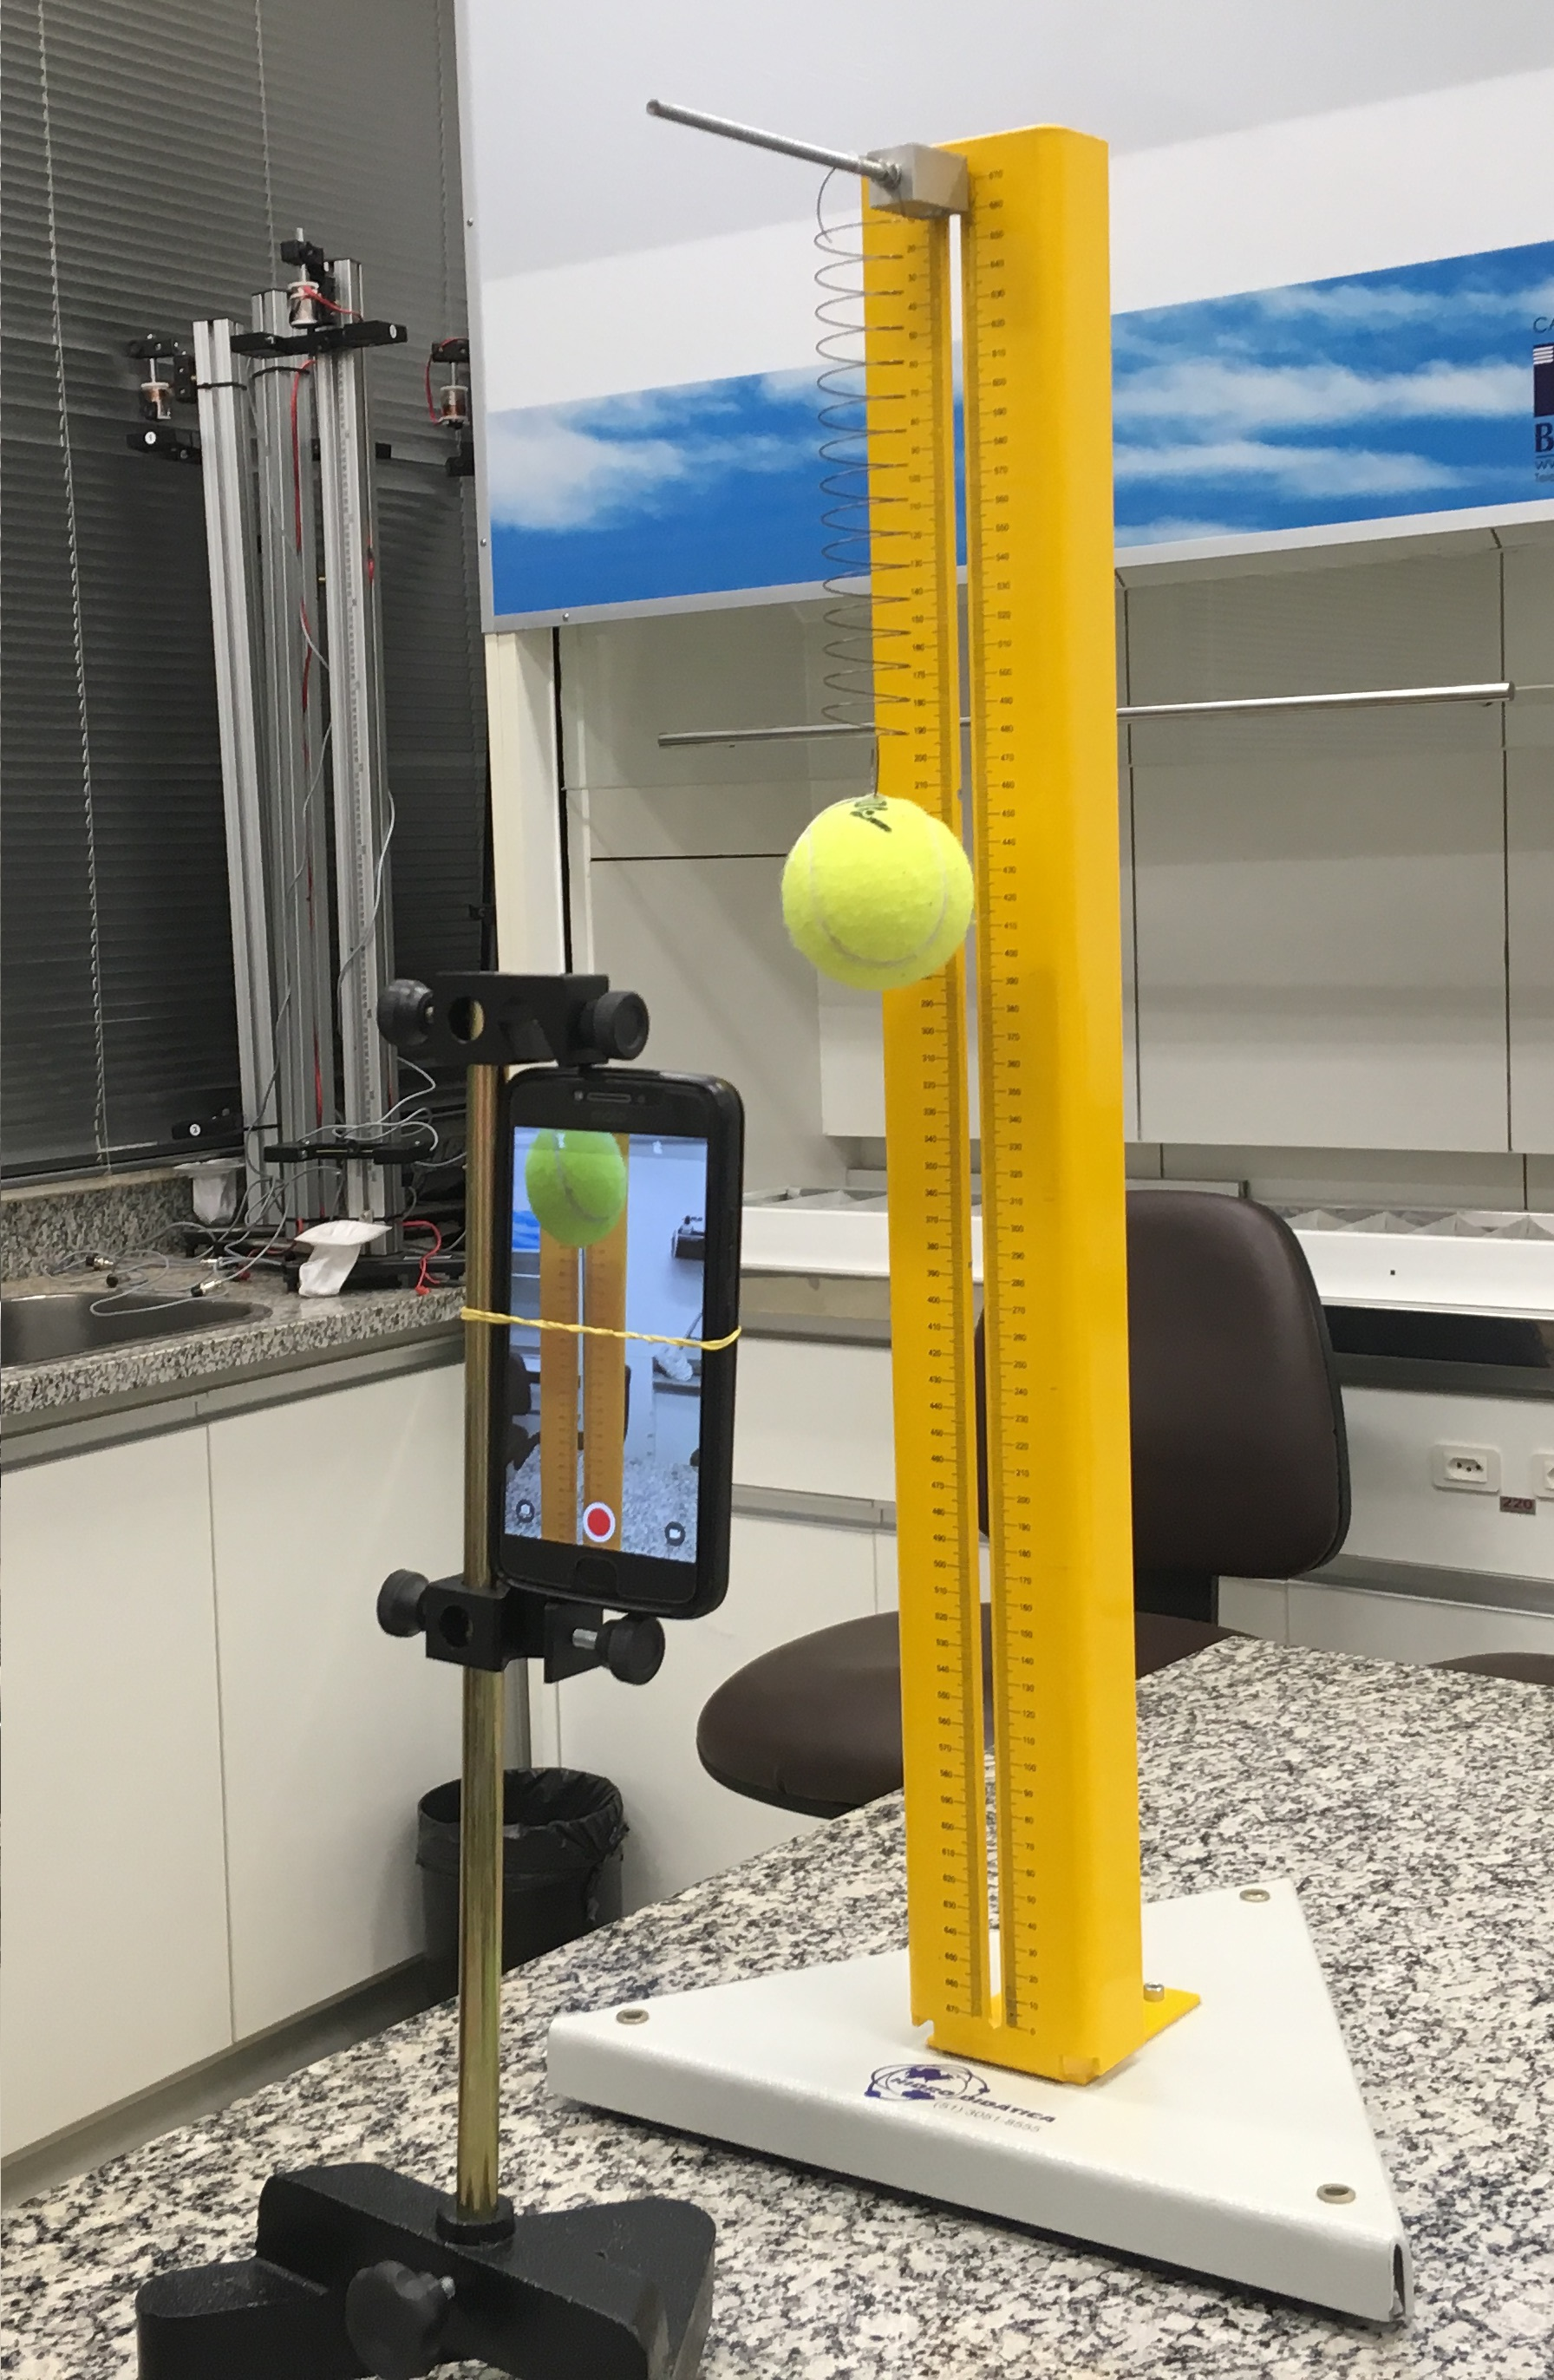
\includegraphics[scale=0.09]{./img/1a.jpg}
				\captionsetup{labelformat=empty}
				\caption{\textbf{Figura 1:} Experimento com bola de tênis}
			\end{figure}
			\begin{figure}[H]
				\centering
				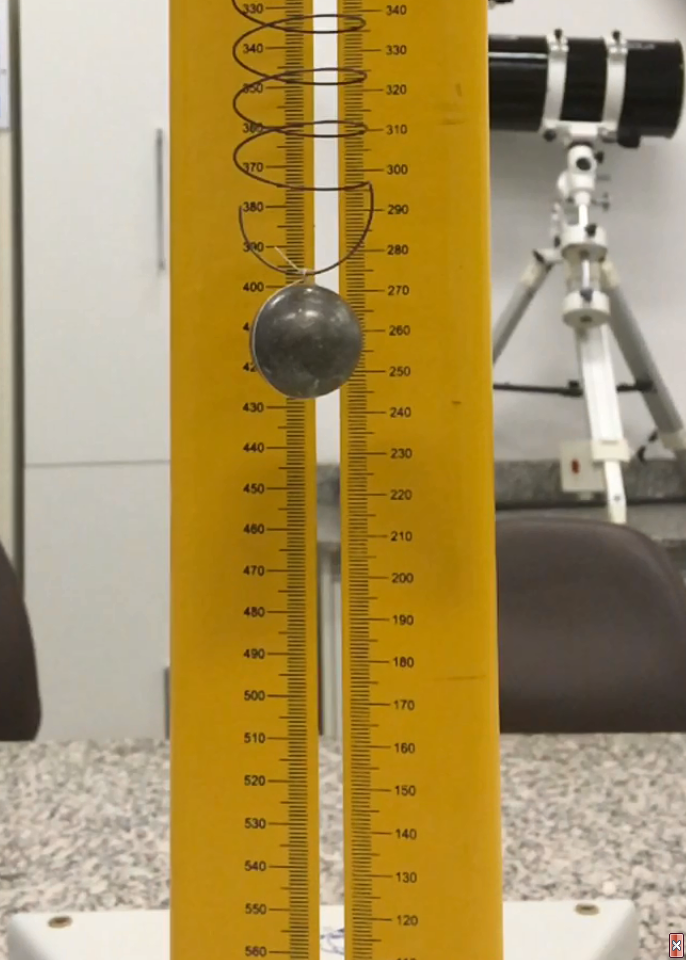
\includegraphics[scale=0.3]{./img/1b.png}
				\captionsetup{labelformat=empty}
				\caption{\textbf{Figura 2:} Experimento com bola de metal}
			\end{figure}
			
		\item \textbf{Análise de Dados}
			\setlength{\parindent}{4ex}
			\par Com os dados da última configuração, fizemos duas análises para determinar o valor da viscosidade do ar: uma utilizando a maior amplitude de cada vídeo curto e outra fazendo a média aritmética das amplitudes máxima e mínima em cada vídeo.
			\par Na primeira análise, tivemos que olhar cada gravação -- quadro a quadro -- para encontrar a maior amplitude e o tempo no cronômetro em que ela foi atingida. Com isso, conseguimos encontrar o valor da viscosidade do ar como $2.78 \cdot 10^{-5} \, Pa \cdot s$ (ignorando as incertezas). Apesar de esse método ter sido efetivo, ele poderia ser mais preciso. Assim, decidimos encontrar valores de amplitudes mais exatos.
			\par Na segunda análise, usamos o programa \textit{Tracker -- video analysis and modelling tool --} para conseguir mais posições em cada vídeo e depois calcular a média aritmética das amplitudes máxima e mínima atingidas nesse intervalo. Como consequência dessa nova análise, conseguimos determinar o valor da viscosidade do ar como $2.02 \cdot 10^{-5} \, Pa \cdot s$ (ignorando a incerteza novamente).
			
		\item \textbf{Conclusão}
		
		\item \textbf{Referências}
		
	\end{enumerate} \end{multicols}
\end{document}